\documentclass[11pt, oneside]{article} 
\usepackage{geometry}
\geometry{letterpaper} 
\usepackage{graphicx}
	
\usepackage{amssymb}
\usepackage{amsmath}
\usepackage{parskip}
\usepackage{color}
\usepackage{hyperref}

\graphicspath{{/Users/telliott_admin/Tex/png/}}
% \begin{center} 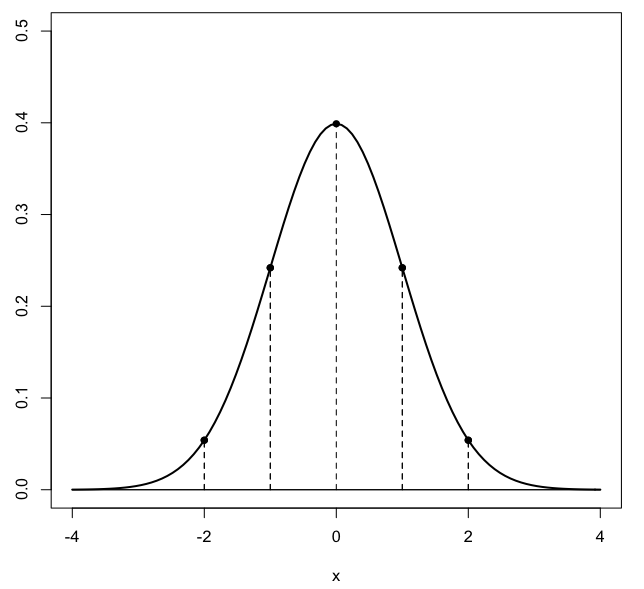
\includegraphics [scale=0.4] {gauss3.png} \end{center}

\title{Folded paper}
\date{}

\begin{document}
\maketitle
\Large

\subsection*{movie screen}
A movie screen on a wall is 20 feet high and 10 feet above the floor. At what distance x from the front of the room should you position yourself so that the viewing angle $ \theta $ of the movie screen is as large as possible ?
\begin{center} 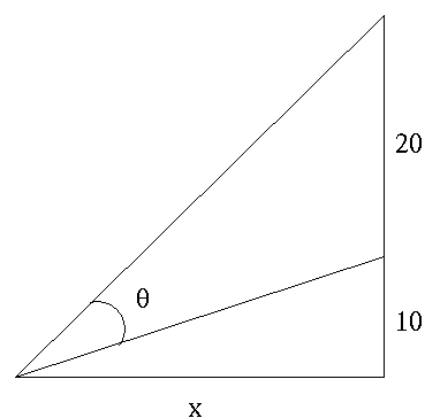
\includegraphics [scale=0.4] {movie_screen.png} \end{center}

Somehow we need to maximize $\theta$ as a function of $x$, but we are given values that form the tangent of two angles.

However, we know that for $\theta$ in the half-open interval $[0, \pi/2)$, as $\theta$ increases so does $\tan \theta$.  Therefore, if we maximize $\tan \theta$, then $\theta$ will also be a maximum.

Let's use $s$ for the entire angle and $t$ for the lower triangle, then
\[ \theta = s - t \]
and the values we were given correspond to the tangents of $s$ and $t$.

We derived $\tan s - t$ before, and can do it again:
\[ \tan s - t = \frac{\sin s - t}{\cos s - t} \]
\[ = \frac{\sin s \cos t - \cos s \sin t}{\cos s \cos t + \sin s \sin t} \]
\[ = \frac{\tan s - \tan t}{1 + \tan s \tan t} \]

Plugging in the values provided:
\[ \tan \theta = \tan s - t = \frac{30/x - 10/x}{1 + 300/x^2} \]
\[ = 30 \ \frac{x}{x^2 + 300} \]
We take the derivative and set it equal to zero.  We can ignore the leading factor of $30$, obtaining
\[ 0 = \frac{x^2 + 300 - 2x^2}{(x^2 + 300)^2} = \frac{-x^2 + 300}{(x^2 + 300)^2} \]

This is equal to zero when the numerator is zero, that is, when
\[ x = \pm \sqrt{300} \]
Since $x$ is a distance we take the positive square root.
\[ x = \sqrt{300} = 10 \sqrt{3} \]

The angles are worth working out.  The tangent of the lower angle $t$ is $1/\sqrt{3}$.  This is a right triangle with hypotenuse equal to $2$ and sine equal to $1/2$.  Therefore $t = \pi/6$.

The tangent of the entire angle $s$ is equal to $3/\sqrt{3} = \sqrt{3}$.  This is a right triangle with hypotenuse equal to $2$ and cosine equal to $1/2$.  Therefore $s = \pi/3$.  

Therefore the angle to the screen $\theta = s - t$ at the maximum is $\pi/6$ or 30 degrees.

\subsection*{folded paper}

Consider a piece of paper with the dimensions $6 \times 12$.  We pick up the lower right-hand corner and place it against the left side, folding to form a crease.

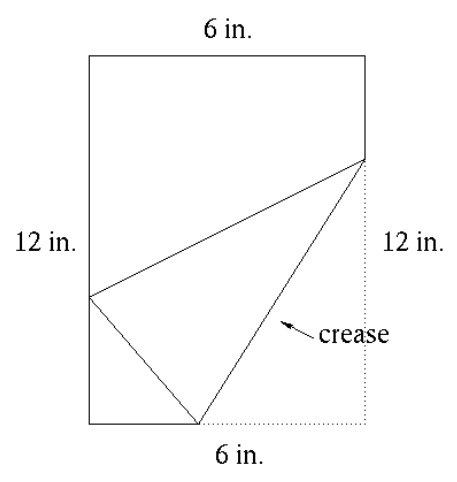
\includegraphics [scale=0.4] {folded_paper1.png}
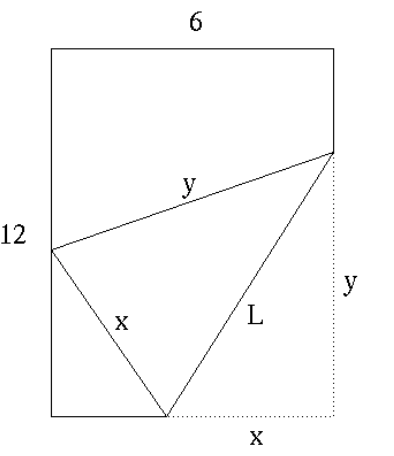
\includegraphics [scale=0.4] {folded_paper2.png}

The possible positions on the left-hand side to place that corner range from the bottom up to a distance 6 inches above the bottom.  The length of the crease is a variable, and and we wish to find the crease with the minimum length.

The variable distances can be labeled as shown on the right.  The length $L^2 = x^2 + y^2$.

I notice that the drawing is not properly scaled (the long dimension is too short).  In fact, the angle that the folded part makes on the left-hand side is a right angle.  After all, it is a corner of the original sheet, but also we have two congruent triangles, they must both be right triangles.

\begin{center} 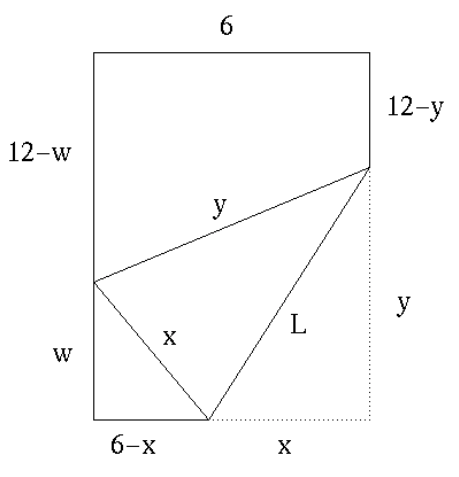
\includegraphics [scale=0.4] {folded_paper3.png} \end{center}
At this point, I notice that the problem can be re-scaled so the length of the paper is $2$ and the width is $1$, in order to simplify the arithmetic.  I have not re-done the drawings to reflect that yet, but our math will take advantage of it.

The range of the distance $x$ is $[1/2,1]$, while that for $y = [1,2]$.

We need to find a relationship between $x$ and $y$.  Start by labeling another variable distance $w$, as shown above.  

The connection that we need can be found by relating $x$, $y$ and $w$ to the total area of the paper.  We have two right triangles with sides $x$ and $y$ and total area $xy$.  

The other triangle has
\[ w^2 = x^2 - (1 - x)^2 \]
\[ = 2x - 1 \]
\[ w = \sqrt{2x - 1} \]
and area (we leave $w$ as it is for now).
\[ \frac{1}{2} (1-x) w  \]
We will need it later, so let's get the derivative of $w$ with respect to $x$
\[ \frac{dw}{dx} = \frac{1}{\sqrt{2x - 1}} = \frac{1}{w} \]

Last, we have a rhombus.  The average of the two vertical sides is 
\[ \frac{1}{2} (2 - w + 2 - y) = 2 - \frac{1}{2} (w + y) \]
and since the horizontal side is $1$, this is also equal to the area.

\subsection*{area calculation}

From the dimensions of the paper, the total area is $2$ and this is equal to the three triangles and the rhombus added together
\[ 2 = xy + \frac{1}{2} (1-x) w  + 2 - \frac{1}{2} (w + y)  \]
\[ 4 = 2xy + (1-x)w  + 4 - w - y \]
Cancel the $4$ and gather terms with $y$ on the left:
\[ y - 2xy =  -y(2x - 1) = -yw^2 \]
So
\[ -yw^2 = (1-x)w - w \]
Factor out one $w$
\[ -yw = (1 - x) - 1 = -x \]
\[ y = \frac{x}{w} \]

That's a nice simplification.  We can check that this is correct at one extreme.  When $x = w = 1$ the ratio is $1 = y$ and we see that is correct for the fold at 45 degrees.  At the other extreme we have $w = 0$ and the ratio is undefined.

Now, minimize $L$
\[ L = x^2 + y^2 \]
\[ = x^2 + \frac{x^2}{w^2} \]
\[ = x^2 + \frac{x^2}{2x - 1} \]
Take the derivative:
\[ \frac{dL}{dx} = 2x + \frac{2x (2x - 1) - x^2 (2)}{(2x -1)^2} \]
Set it equal to zero and factor out $2x$:
\[0 = 1 + \frac{(2x - 1) - x}{(2x -1)^2} \]
\[ (2x - 1)^2 + x - 1 = 0 \]
\[ 4x^2 - 3x = 0 \]
Factor out another $x$
\[ 4x - 3 = 0 \]
\[ x = \frac{3}{4} \]
The minimum crease length occurs when $x$ is halfway along its range.

I found the last two problems here:

\url{https://www.math.ucdavis.edu/~kouba/CalcOneDIRECTORY/maxmindirectory/MaxMin.html}

\end{document}